\chapter{Background}
\label{sec:metrics}

This chapter describes background knowledge required to understand the remaining parts of the thesis. It introduces the target system for this work as well as datasets and metrics used for evaluation. Furthermore, it discusses related work in Object Detection and Data Generation.

\section{System Environment}

A \ac{MAV} consist of multiple components of Software that are responsible for higher and lower level tasks. \Cref{fig:control_loop} illustrates these components in the example of the target platform of this thesis. On the lowest level drivers read out sensors such as the camera and an \ac{IMU} or communicate with a ground station. A low level control loop is responsible for controlling the local state of the \ac{MAV} such as altitude and attitude. A higher level control loop controls the global state of the \ac{MAV} which is the position and the flying trajectory.


\begin{figure}[hbtp]
	\centering
	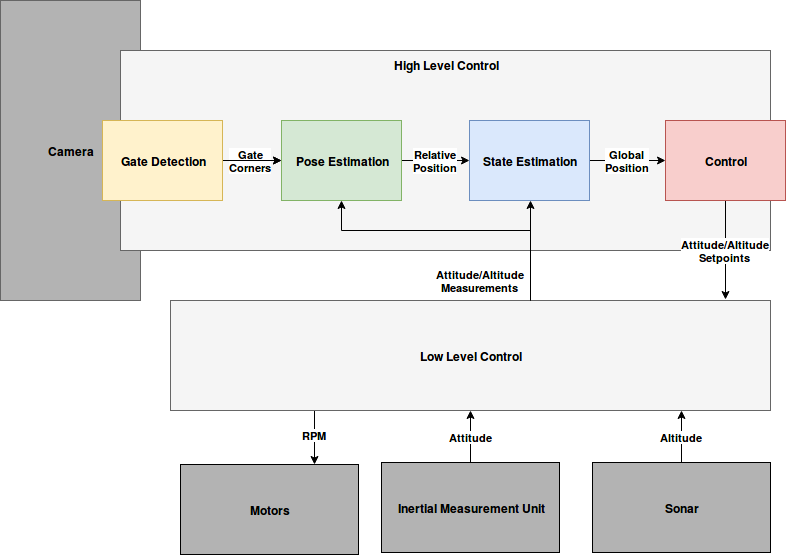
\includegraphics[width=0.8\textwidth]{fig/control_loop}
	\caption{Control Loop}
	\label{fig:control_loop}
\end{figure}

The high level control loop how it is targeted in this work is described further detail. A first step detects the racing gate and yields the corner coordinates. These are used to estimate the relative position of the \ac{MAV} towards the gate. In the third step the visual measurements are fused with measurements of other sensors. In the case of this work \ac{IMU} and a sonar deliver altitude and attitude data. This step yields a global position estimate of the \ac{MAV}. Based on this estimate a flying trajectory is calculated. This results in desired altitude and attitude which is send as set points to the low level controller.

The hardware platform used to run the high level control loop is the \textit{JeVois} smart camera. It contains a 1.3 MP camera with 65 degree field of view. The processing units are a quad core ARM Cortex A7 processor with 1.35 GHz and a dual core MALI-400 GPU with 233 Mhz. In order to extent the field of view a 120 degree wide angle lens is mounted. In \Cref{fig:jevois} the camera is shown.

\begin{figure}[hbtp]
	\centering
	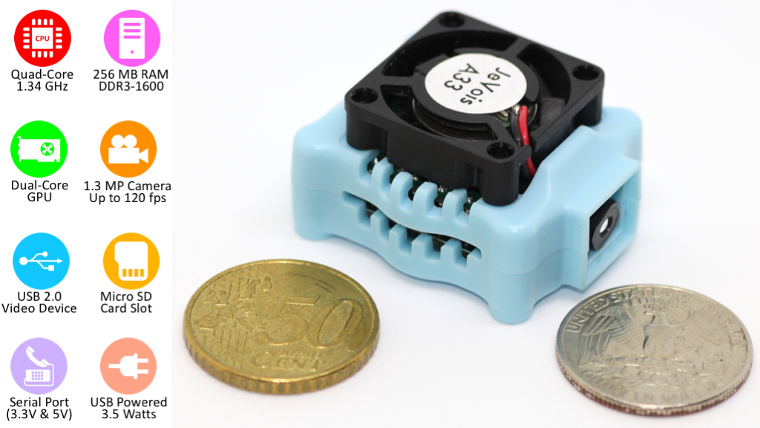
\includegraphics[width=0.5\textwidth]{fig/jevois}
	\caption{JeVois Camera}
	\label{fig:jevois}
\end{figure}

\subsection{Baseline Algorithm}

The baseline algorithm \textit{SnakeGate} is a low-level image processing algorithm proposed in \todoref{snakegate}. Its scheme is summarized in and described in the following.

\begin{enumerate}
	\item Filter image by colour threshold
	\item Sample stochastically 
	\item Follow the pixels horizontally as long as they are within the colour threshold otherwise return to 2.
	\item If a bar of sufficient length has been found repeat 3. vertically along one end of the line found in 3.
	\item If a vertical bar is found the square is considered as gate candidate
	\item Create local histogram around the corners of the gate candidate and choose the highest peak as gate corner.
	\item Count the fraction of pixels within the color threshold  in relation to the total number of pixels a long all edges of the gate candidate to determine the \textit{color fitness}.
	\item Gate candidates that exceed a chosen threshold are considered valid detections.
\end{enumerate}
\todo{this can be described more formally}

A property of SnakeGate is that it can and has to be fine tuned given an environment and its corresponding light conditions. This lack of robustness against domain changes are one motivation for this work. On the other hand, in practice the fine tuning allows to adapt the method live for a certain domain, which is not practical for learning based methods.



\section{Datasets}
\label{sec:datasets}
An evaluation set has been recorded to serve as a benchmark for the developed methods. The dataset consists of 300 images recorded with the JeVois camera during flight and while remaining on ground. The samples stem from three different rooms with varying light conditions. The rooms are referred to as \textit{Basement}, \textit{Cyberzoo} and \textit{Hallway}. Example images for each room can be seen in \Cref{fig:example_real_set}.
\begin{figure}
	\centering
	\begin{minipage}{0.3\textwidth}
		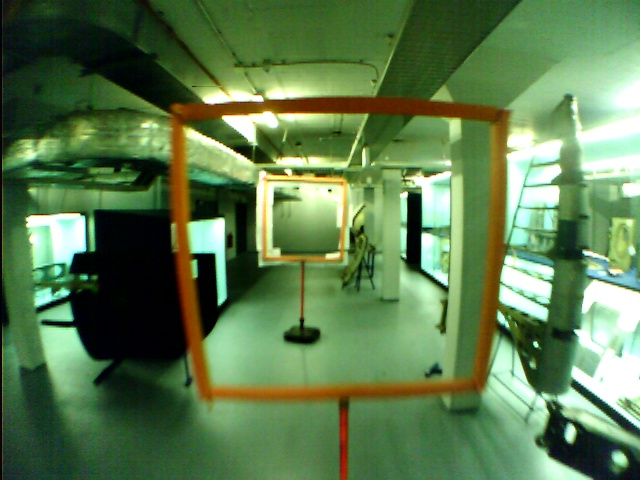
\includegraphics[width=\textwidth]{fig/basement}
	\end{minipage}\hfill
	\begin{minipage}{0.3\textwidth}
	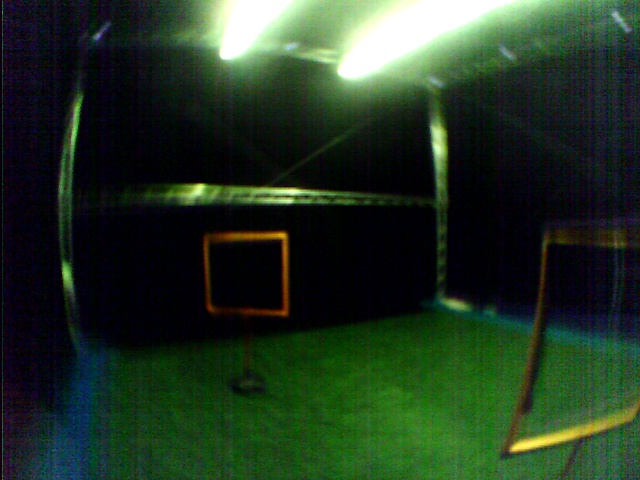
\includegraphics[width=\textwidth]{fig/cyberzoo}
\end{minipage}\hfill
	\begin{minipage}{0.3\textwidth}
	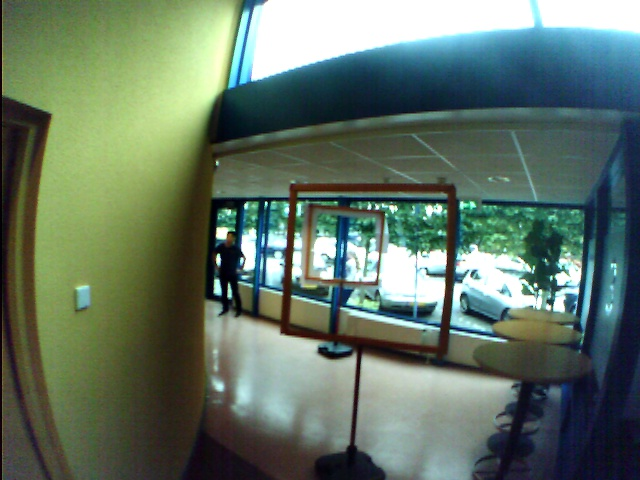
\includegraphics[width=\textwidth]{fig/hallway}
\end{minipage}
\caption{Examples of the three test domains. From left to right: \textit{Basement}, \textit{Cyberzoo} and \textit{Hallway}}
\label{fig:example_real_set}
\end{figure}

All scenes are indoor scenes which are a typical example for a GPS-denied area, where vision based state estimation is required. The scenes contain two gates that are arranged in varying order. Hence up to two objects are visible and can overlap which means the gate farer away can be seen through the closer gate. Each of the rooms has different environmental conditions:
\begin{enumerate}
	\item \textit{Basement} is a bright environment illuminated by artificial light sources. The corridor in which the objects of interest are placed are narrow while also objects and persons are visible on the samples. The dataset contains 163 samples with 312 objects in total.
	\item \textit{Cyberzoo} is taken from a test environment for drone flights. External light sources are covered such that an even illumination and dark background is created. Only in a small subset of images distractors like other objects or persons are visible. In total 88 samples stem from this room while 71 objects are present.
	\item \textit{Hallway} is a bright environment illuminated by a combination of artifical light sources as well as daylight that shines through the windows. The samples are taken with the windows as background. This leads to a very bright background such that the thin structure of the objects are hardly visible. The dataset contains 49 samples with a total of 86 objects.
\end{enumerate}

\section{Evaluation Metrics}

The detection performance is evaluated in terms of precision and recall. These metrics are defined as:

\paragraph{Precision}
$$p = \frac{\text{true positives}}{\text{true positives} + \text{false positives}}$$

\paragraph{Recall}
$$r = \frac{\text{true positives}}{\text{true positives} + \text{false negatives}}$$

Where true positives are objects that are detected, false positives are detections although there is no object and false negatives are objects which have not been detected.

Hence, recall expresses how many of all objects are detected and therefore how complete the result is. Precision measures how many of the predicted objects are actually correct detections.

A correct detection is determined based on its overlap with a ground truth box. This is measured by the relation of \ac{IoU}. In experiments we determine 0.6 as sufficient overlap for a detection. However, to evaluate how accurate in terms of location the detections are, precision and recall are measured for different levels of \ac{IoU}.

The model used within this thesis associates a "confidence" value with each prediction that can trade off precision and recall. This is further explained in \Cref{sec:object_detection}. By accepting more detections with a lower confidence threshold, the probability increases that one of the predictions is a true positive. Hence, it increases recall. However, it also increases the probability of false positives and thus lowers precision. In order to evaluate this trade-off precision is plotted over recall at increasing confidence values.

As the learning of \acp{CNN} is stochastic, the mean across several trainings is reported. In order to determine the average precision recall trade-off the precision is interpolated across evenly distributed recall levels between 0 and 1 using:

$$ p_\text{interp}(r) = \max\limits_{r' \geq r} p(r')$$

Subsequently the mean at all recall levels can be calculated. A metric that combines the precision-recall trade-off is \ac{mAP}:


$$ mAP = \int_{r}p_{interp}(r) dr$$

\todoref{There should be a source for this}

\section{Related Work}

\subsection{Object Detection}
\label{sec:object_detection:related}
The existing methods can broadly be grouped in three groups. Those are more traditional approaches without \acp{CNN}-based feature extraction, two-stage detectors and one-stage detectors.

\subsubsection{Traditional Methods}

One of the first object detection methods was \cite{Viola2004} that used simple filters inspired by Haar-basis functions as a feature extractor for human face detection. The image was processed in a cascade of classifiers that assigned the label "face" or "background" to image patches. The output of the first stages were further classified when going deeper in the cascade. The processing of one image patch stopped, when a classifier assigned the label "background". Although being very fast the Haar-based feature extraction is not very robust towards rotation-, scale- or shape-variations \todo{quote}. 

A more robust feature extractor was proposed by \cite{Dalal} and \cite{Lowe2004} for pedestrian detection. A local (normalized) histogram of gradients is computed for a fixed window size. 

Previously mentioned methods modelled objects as one instance. This prove to be sensitive towards part occlusions or large deformations. Deformable part models detect object parts individually and combine them. Thus a feature extractor can still give a high response when even only object parts are visible or they are arranged in a way untypical to the training set.

Guido proposes a neural network to learn an attention model.

X propose a recurrent neural network architecture to model the attention process.

\todo{discussion traditional features}

\subsubsection{\acp{CNN}-based Feature Extraction}

In recent years \acp{CNN} emerged from Deep Learning research and became a popular feature extractor. \acp{CNN} can be seen as small neural networks that are applied locally on image patches in sliding window fashion. The outputs of the initial local operations (first layer) are further processed by higher layers until the desired output size is reached. The model parameters (weights) are trained using a Loss function and the back-propagation algorithm.

The modular structure of \acp{CNN} allow to create highly non-linear models that can represent any function. However, this flexibility also introduces the challenge of choosing a suitable architecture. On a fundamental level design parameters can be summarized in depth, width and kernel size. 

\Cref{fig:model_design} displays these parameters and introduces additional terminology necessary for the remaining parts of this chapter. The \textit{kernel size} $\textbf{k}$ determines the spatial size of a kernel and therefore how big the patch is, the convolution is applied on. A layer usually contains multiple filters that are applied on its input. The amount of filters is also referred to as \textit{width} $w$. The filters are applied in sliding window fashion which introduces the step size ( \textit{strides} $\mathbf{s}$) as an additional parameter. The output of each convolution is concatenated and processed by the next layer. The amount of layers is also referred to as \textit{depth}. In the image also the \textit{receptive field} of a filter is visualized. This describes the image patch that is related to a certain feature response. The filter of the first layer (green) has a receptive field corresponding to its kernel size. The filter of the second layer (blue) combines the responses of the filters of the first layer at multiple spatial locations an thus has an increased receptive field.

\begin{figure}[hbtp]
	\centering
	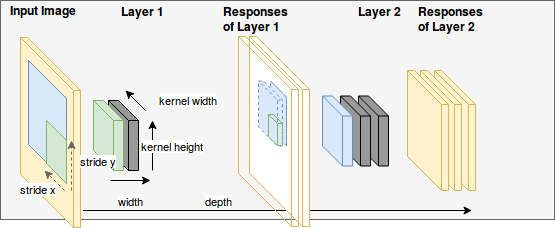
\includegraphics[width=0.8\textwidth]{fig/model_design}
	\label{fig:model_design}
	\caption{Example Architecture of a \ac{CNN}}
\end{figure}

Among these parameters depth is considered one of the preliminary parameters to improve performance \cite{He}. \citeauthor{Simonyan2014} \cite{Simonyan2014} achieve first places in the 2014 ImageNet Classification challenge using a network that only contained filters of size 3-by-3 but up to 19 layers. \citeauthor{Szegedy2014} \cite{Szegedy2014} achieve similar performance using a network with 22 layers. The proposed network included a \textit{Inception}-module, an architectural element that allows deeper networks at a constant computational budget. 

An issue that prevented training even deeper networks is the \textit{vanishing gradient problem}. As the gradient distributes while flowing through the vast amount of nodes its magnitude gets very small. Hence, the training becomes slow and the risk of converging in a local minima increases. This was addressed by \citeauthor{He2015} \cite{He2015} who propose the use of residual connections. Instead of propagating the gradient from the last to the first layer these connections allow the gradient to flow directly into all layers. This circumvents the vanishing gradient problem. The use of residual connections allowed to train a network 101 layers and improved on state of the art at that time.

However, later work by \citeauthor{Zagoruyko2016} \cite{Zagoruyko2016} shows how residual networks do not behave like a single deep model but more like an ensemble of more shallow networks. Moreover, the study shows that similar performance can be achieved by particularly wide networks and residual connections. Being of similar performance the proposed \acp{WRN} are computationally more efficient to execute.

While wide residual networks can achieve similar performance to deep residual networks with reduced inference time the computational requirements are still large. This work addresses the detection of \ac{EWFO} with very limited resources. Hence, a network in which the vanishing gradient problem would appear is likely to be already too computationally expensive to be applied on a \ac{MAV}.

Instead the work focuses on much smaller networks that are fast to execute. Execution time is also the motivation for \acp{FCN}. Instead of using a fully connected layer in the last stage, these network only apply local operations. This saves many computations in the last layer and enables the application of models on various input sizes.

However, \ac{FCN} in combination with a small amount of layers introduce a limited receptive field. A way to increase the receptive field without increasing the number of computations was proposed by Atrous/Dilated convolutions consist of a sparse kernel thereby increasing the receptive field of a filter without increasing complexity or number of computations \todoref{Atrous}.

Despite a large amount of research conducted in finding suitable architectures there has not yet been a single way that always achieves a goal. It has been shown how models with a large amount of parameters combined with huge training data perform well on various vision tasks and objects. However, there is no guarantee that the found representation is also the most suitable/efficient one. The research resulted in a collection of rules an best practices that need to be considered with the task at hand. This work investigates the design of a \ac{CNN} for the detection of \ac{EWFO}.

\subsubsection{\ac{CNN}-based Object Detection}

\acp{CNN}-based feature extraction is employed in various approaches to Object Detection. 	

\citeauthor{Girshick2013} \cite{Girshick2013} use the Selective Search algorithm \cite{Uijlings2013} to extract object candidates from an image and classify each region with a \ac{CNN}. However, this requires to run the whole network at various scales and overlapping locations. Hence, the approach contains a lot of redundant operations and is computationally intense.

\citeauthor{Ren} \cite{Ren} use a \ac{RPN} to propose regions that likely contain an object. In order to define the proposal task as a regression problem, the approach introduces so called \textit{anchor boxes}(also \textit{prior boxes}, \textit{default boxes}). These are boxes of predefined size and location. The model predicts class probabilities and coordinate offsets for each of these boxes. Hence, a certain set of output nodes is responsible for a particular box. If during training a ground truth box has sufficient overlap with a certain box the corresponding output nodes are assigned "responsible" to predict that object. That means the loss is only propagated via those nodes. 

\Cref{fig:anchors} illustrates the concept. The anchor boxes are displayed as dashed lines while the ground truth is displayed solid. The ground truth box in blue has sufficient overlap with two anchor boxes. Hence, these two sets of output nodes take part in the loss calculation. In the example each of these sets predicts coordinate offsets $\Delta(cx, cy, w,h)$ and class probabilities $c_1 .. c_p$.

\begin{figure}[hbtp]
	
	\centering
	\captionsetup{justification=raggedright,singlelinecheck=false}
	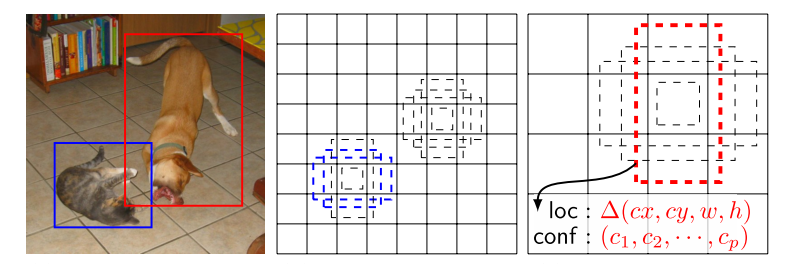
\includegraphics[width=0.8\linewidth]{fig/anchors}
	\caption{Visualization of the anchor box concept \cite{Liu}.}
	\label{fig:anchors}
	
\end{figure}

For the classification stage an \ac{SVM}-classifier is used. The classifier is trained on the image patches extracted by the first stage. \acp{RPN} enabled to propose multiple candidate regions with a single inference of the network. Thus, the expensive feature extraction stage is run only once which results in a significant speed up \todo{how much?}. A drawback is the fact that individual stages of the method have to be optimized individually. Furthermore, the training requires to store large amounts of extracted patches on the hard drive.

In the follow up work \cite{Ren} propose the \textit{ROI}-pooling layer. The layer uses spatial pyramid pooling in order to resize region proposals to a fixed size. This enabled the end-to-end training of the two-stage detection pipeline. \todo{And resulted in?}

Another end-to-end pipeline was published by \citeauthor{Redmon} \cite{Redmon}. In contrast to aforementioned approaches, the network performs Classification and Localization in a single pass. The task is formulated by dividing the input image in a fixed grid and predicting $C$ class probabilities for each grid cell. Additional $5*B$ output nodes predict $B$ set of bounding box coordinates and $B$ object probabilities for each cell. \todo{what is good and bad?}

\citeauthor{Liu} propose \ac{SSD} \cite{Liu}, one stage detector using the concept of aforementioned anchor boxes. Instead of only predicting an object score for each anchor box, the model also predicts class probabilities. Another novelty in this approach is the use of multiple predictor layers for various scales. The network does not only use its final layer for prediction but also intermediate representations. Assuming that the lower layers preserve more fine grained features, early output nodes are trained on smaller objects while later output nodes focus on predicting larger scale objects.

Follow up work of \citeauthor{Redmon}\cite{Redmon, Redmona} also included the concept of anchor boxes and prediction layers at multiple scales, making \ac{SSD} and \ac{Yolo} converge to a very similar solution. A novelty in \cite{Redmona} is the use of de-convolution layers for small object prediction. In order to achieve a higher accuracy for small objects the final layers are up-sampled and combined with finer grain features from earlier layers. The aim is to enable a combination of deep semantic features at low spatial resolution with fine grain low level features at high resolution.

Within the framework of \ac{SSD} and \ac{Yolo} several approaches exist that either change the base network or modify layers in between: \cite{ChengchengNing2017} propose propose a more efficient non-max-suppression method as well as to include an inception module in the network architecture to reduce computation while keeping/increasing performance. \cite{Wu} uses \textit{SqueezeNet} as base network and a mixture between the ssd and yolo loss function as training goal. \cite{Xiang} investigates the receptive fields of SSD and tries to incorporate more context, especially on lower feature maps, to increase detection rate for small objects.\cite{Linb} applies the framework for vehicle detection. They use \textit{GoogLeNet} as base network (and investigate several others).\cite{TripathiSanDiego} apply a network very similar to YoloV2 and investigate 8bit quantization of the model to make it runnable on embedded devices.

A common problem of one stage detectors is the imbalance between background and object samples. Most methods upweigh the positive samples and/or use hard negative mining. \cite{Lin} introduces the \textit{Focal Loss} which focuses on sparse positive samples by design.

\todoref{CornerNet}


Each of the described group of methods has strengths and weaknesses. While shallow methods are typically quite fast they require a lot of manual effort and/or are not so accurate. Two-stage detectors on the other hand are quite accurate but their computational requirements are prohibitive for the hardware to be used in this thesis. One-stage detectors offer a compromise between detection accuracy and inference speed. In addition they can be trained end-to-end which requires only little manual engineering. However, the presented methods are still too slow for the hardware used in this thesis.




%			\paragraph{Scalable Object Detection using Deep Neural Networks\cite{Erhan}}
%			\begin{itemize}
%				\item[-] Generates number of bounding boxes as object candidates (class agnostic) and confidences for each box
%				\item[-] For each Bounding Box a classifier is run e.g. DNN
%				\item[-] Training: If the number of boxes k is larger than the number of objects b, only b boxes are matched while the confidence of the others is minimized
%				\item[-] Assignment problem $$F_{match}(x,l) = \frac{1}{2}\sum_{i,j}x_{ij}||l_i - g_j||^2_2$$ where $x_ij$ is one if the ith prediction is assigned to the jth ground truth object
%				\item[-] Confidence: 
%				$$F_{conf}(x,c) = - \sum_{i,j}x_{ij}*\log(c_i)-\sum_{i}(1-\sum_{j}x_{ij})\log{1-c_j}$$
%				\item[-] Speed up training by clustering (kmeans) of ground truth and using it as prior (prior matching)
%				\item[-] Can be defined to output boxes only for a particular class by training the bounding boxes on that class
%				\item[-] Number of parameters grows linearly with number of classes
%				\item[-] Authors argue two step process (region proposal + classification) is better
%				\item[-] Architecture based on AlexNet
%				\item[-] Predicted boxes are merged using non-maxima surpression
%				\item[-] One shot(50\%), +2scales (75\%)
%				\item[-] OverFeat/ Selective Search are faster but much more expensive
%			\end{itemize}




\todoref{Wire detection}

\subsection{Data Generation}
\label{sec:training:related}

Related methods vary from changing low level properties of the image over using CAD models in combination with real background up to rendering full 3D-environments. Often various combinations of synthesized and real data are applied. 

\subsubsection{Low-Level Image Augmentation}

A common part of current Computer Vision pipelines is to augment a given data set by transforming low level properties of the image. By artificially increasing variations in the input signal, a model that is more invariant to the augmented properties shall be obtained.

\citeauthor{Krizhevsky2012a} \cite{Krizhevsky2012a} use \ac{PCA} to incorporate colour variations. \citeauthor{Howard2013} \cite{Howard2013} shows how several image transformations can improve the performance of a \ac{CNN}-based Classification model. The proposed pipeline includes variations in the crop of the input image as well as variations in brightness, color and contrast. In \ac{CNN}-based Object Detection \citeauthor{Redmon} \cite{Redmon} uses random scaling and translation of the input image, as well as random variations in saturation and exposure. \citeauthor{Liu} \cite{Liu} additionally crop and flip each image with a certain probability.

Since most methods use image augmentation and \citeauthor{Krizhevsky2012a} \cite{Krizhevsky2012a} mentions it to be the particularly reason for superior performance at ILSVRC2012 competition it can be assumed to be beneficial for Computer Vision models. Unfortunately, none of the publications measures the improvements gained by the different operations. 

While the aforementioned approaches add artificial variation to the input data, \citeauthor{Carlson2018}\cite{Carlson2018} augment the image based on a physical camera model. The proposed pipeline is applied for Object Detection and incorporates models for sensor and lens effects like chromatic aberration, blur, exposure and noise. While being of minor effect for the augmentation of real data (0.1\% - 1.62\% \ac{mAP}70) the reported results show an improvement when training on fully synthesized datasets. Here the reported gains vary between 1.26 and 6.5 \% \ac{mAP}70.

Low-level image augmentation is a comparatively cheap method to increase the variance in a dataset. However, it cannot create totally new samples or view points. Furthermore, it cannot change the scene in which an object is placed. Therefore it needs a sufficiently large base dataset that is augmented. This work addresses the case when no real training data is available. Hence, low-level image augmentation is incorporated in the training process but can not be the only method applied.

\subsubsection{Augmenting Existing Images with CAD - Models}

In order to create new view points \ac{CAD}-models can be used. These models describe 3D-shape of an object and can be placed on existing images to augment or increase a dataset.

\citeauthor{Peng}\cite{Peng} study the use of \ac{CAD}-models in the context of \ac{CNN}-based Object Detection. The authors particularly address how image cues like texture, colour and background affects the detection performance. The experiments show how the used \acp{CNN} are relatively insensitive towards context but use shape as primary, texture and colour as secondary most important features. This enables competitive performance even when the object of interest is placed only on uniformly covered backgrounds. However, the study only covers solid objects such as birds, bicycles and airplanes. \ac{EWFO} are substantially different and we hypothesize that other image cues must be relevant.

\citeauthor{Madaan2017}\cite{Madaan2017} study the segmentation of wires based on synthetic training. As wires similarly to \ac{EWFO} only consist of thin edges, the application is quite close to this work. However, the experiments focus on a single domain, namely sky images and thus the variations in background are comparatively small. We hypothesize that \ac{EWFO} are particularly sensitive to such variations and address the application in multiple domains.

\citeauthor{Hinterstoisser2017} \cite{Hinterstoisser2017} propose to use a base network that has been trained on real images and to continue training on images with \ac{CAD}-models. During training the base network is frozen and only the last layers are updated. The method does not use real data but requires a suitable base network. As most available feature extractors (further discussed in \Cref{sec:object_detection}) are of a size that is computationally prohibitive for \ac{MAV} the method is not really applicable for this work. 

The use of CAD-models in combination with real backgrounds allows to generate totally new view points for the object of interest. Furthermore, the image background consists of real data and thus the synthetic textures only concern the rendered object. However, the geometric properties like perspective as well as the physical properties like object placement are violated and therefore create an artificial scene. Despite this fact, literature shows that such images can benefit model performance in various cases. Yet, most of the approaches still use real data and/or focus on solid objects with rich textures and complex shape. We hypothesize that since \ac{EWFO} do not provide these kind of structures the results do not apply in the same way. Hence, we incorporate the method to generate data and investigate how it can be applied for the detection of \ac{EWFO}.

\subsubsection{Fully Synthesizing Environments}

A more realistic placement of objects can be achieved when fully synthesizing environments.  The object of interest can be placed according to physical laws, shadows fall correctly and geometric properties of an image are followed. However, if the graphical models do not fully capture the details of real world objects, the generated data might look too artificial.

\citeauthor{Johnson-Roberson2016} \cite{Johnson-Roberson2016} use a powerful graphical engine and a highly detailed environment to train an Object Detection model entirely in simulation. The results show an improvement towards data annotated by humans especially when using vast amounts of simulated data. \todo{There should be more examples for this} 

In order to create realistic environments intense manual work is required for the design. In contrast \cite{Sadeghi2016, Tobin2017, Tremblay2018a} use a relatively simple environment but a high degree of randomization to address the reality gap. The aim is to learn an abstract representation by strongly varying textures, light conditions and object locations. \citeauthor{Tobin2017} introduced this technique as \ac{DR}. The drawback of the approach is that a too high degree of randomization may omit pattern in the target domain that could otherwise be exploited by the model. 

This work addresses the generation of data for the detection of \ac{EWFO} on \acp{MAV} in \ac{GPS} denied scenarios. Such scenarios cover a wide range of possible environmental conditions and the images taken from \ac{MAV} cameras are peculiar. Hence the creation of a full environment is investigated in this work. 


\subsection{Transfer Learning}

The field of transfer learning particularly addresses domain shifts in the modelling process. Hence, a common application is the learning from synthetic data.

A common approach in \ac{CNN}-based models is the incorporation of a domain classifier in the model. By augmenting the data with domain labels, the classifier learns to distinguish the two domains. Subsequently a gradient reverse layer is applied and thus the weights are updated in such a way that a domain agnostic representation is learned. Examples of the approach can be found in \cite{Chen2018c} \cite{Xu2017}.

While the aforementioned approaches require labelled samples from the target domain, \citeauthor{Peng2017} \cite{Peng2017} propose to include task-irrelevant samples and a source classifier. As a result no samples of the target domain are required.

While transfer learning provides the theoretical framework as well as methods to deal with domain shifts, it does not allow to generate data. Furthermore, it often requires samples of the target domain. This work addresses the case when no real data is used for training. The field is interesting to be incorporated in the data generation pipeline investigated in this thesis but it can not be used as a start off point. Hence, the use of transfer learning in the modelling process is denoted as future work.

\subsubsection{Generative Adversarial Networks}

\cite{Inoue} 
\todo{write}





\section{Baseline}


\subsection{Experiment}

In order to compare the methods investigated in this thesis a baseline is determined. Therefore SnakeGate is evaluated on the datasets described in \Cref{sec:datasets}. In the experiment the color thresholds of the algorithm are fine tuned to the particular environment. The presented results are averages across 5 runs.


\subsection{Results}

The results in terms of precision and recall are summarized in \Cref{fig:snake_results_real}. It can be seen how the detector performs best in the Cyberzoo domain.

\begin{figure}
	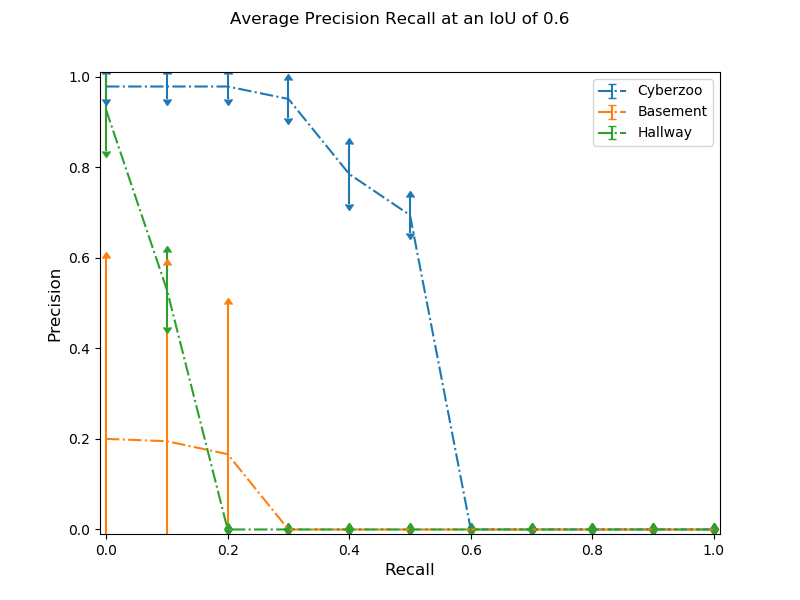
\includegraphics[width=0.8\textwidth]{fig/snake_results_real}
	\caption{Precision-Recall of Snake Gate on the datasets described in \Cref{sec:datasets}}
	\label{fig:snake_results_real}
\end{figure}

